\section{Аналитическая часть}

В данном разделе проводится анализ и выбор методов представления, рендера, преобразования и визуализации твердотельных моделей.

\subsection{Анализ методов представления твердотельных моделей}

Моделирование твёрдого тела --- это последовательный и 
непротиворечивый набор принципов математического и компьютерного 
моделирования трёхмерных твёрдых тел. 
Рассмотрим 
существующие методы представления твёрдых тел.

%\subsubsection{Клонирование примитивов}
%
%TODO зачем вообще нужно оно тут? Может и не нужно? Если нужно, переработать
%Данный метод представления основан на понятии семейств объектов. 
%Семейством называют группу объектов, отличающихся несколькими 
%параметрами друг от друга \cite{cloning}.
%Например, с помощью операций поворота и 
%масштабирования из исходного объекта можно получить семейство (рис. \ref{fig:primitiveClone}).
%
%\begin{figure}[h]
%	\centering
%	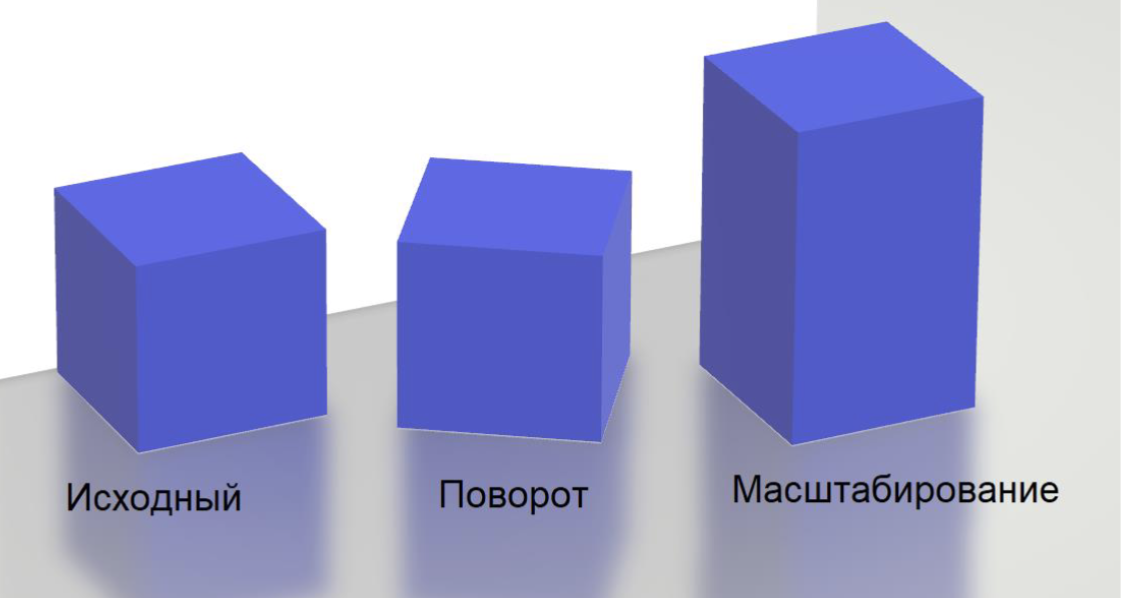
\includegraphics[width=\textwidth]{img/primitiveClone.png}
%	\caption{Пример семейства объектов}
%	\label{fig:primitiveClone}
%\end{figure}
%
%При этом каждое семейство объектов называется общим примитивом, а 
%отдельные объекты называются примитивными экземплярами. 
%Так, семейство гаек является общим примитивом, а конкретная гайка, определённая набором характеристик, является примитивным экземпляром.
%Особенностью данного методы является невозможность создать сложный 
%объект сочетанием экземпляров. 
%
%TODO написание два раза повторяется Минусом данного метода является сложность написания алгоритмов для вычисления свойств представленных тел --- отсутствие возможности написать общий алгоритм из-за уникальности примитивов;
%
%К плюсам можно отнести простоту реализиации агоритма, если требуется представление только конкретного семейства моделей. 
%
%Для решения поставленной задачи необходим метод, который позволит 
%не зависеть от типа модели, её формы и параметров.  
%
%Изучив данный метод, можно заключить, что он не подходит для решения 
%поставленной задачи, так как возникает необходимость в подробном описании 
%всех свойств определённого семейства, что будет проблематично осуществить 
%для составных тел.

\subsubsection{Граничное представление}
В граничном представлении (\textit{англ.} Brep --- Boundary Representation) \cite{brep} твердотельные модели представляются как совокупность 
двумерных границ, которые описывают трёхмерную модель. 
Твёрдое тело описывается как замкнутая пространственная область, ограниченная набором элементарных поверхностей (граней), имеющих образующие контуры (рёбра) на границе и признак внешней или внутренней стороны поверхности (пример представлен на рисунке \ref{fig:brep}). 

\begin{figure}[h]
	\centering
	\captionsetup{justification=centering}
	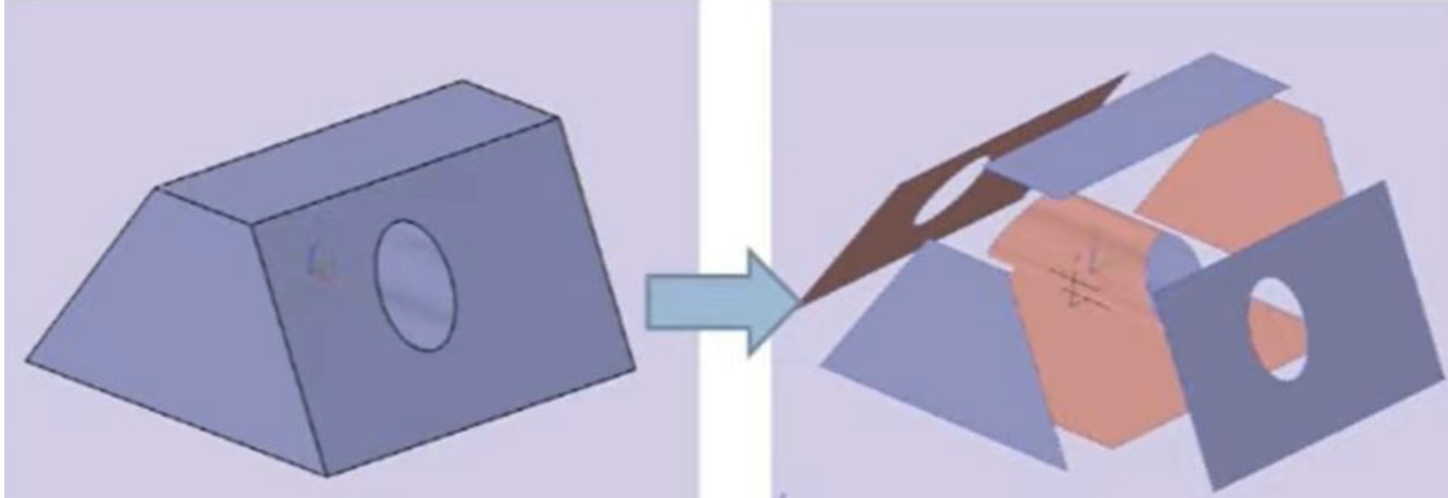
\includegraphics[width=160mm]{img/brep.png}
	\caption{Пример представления твёрдого тела как замкнутой области и набора поверхностей}
	\label{fig:brep}
\end{figure}

Такая схема проектирования крайне распространена в приложениях 
САПР, но, несмотря на это, она также имеет ряд недостатков, которые могут 
привести к проблемам визуализации результата.

Недостатки:
\begin{itemize}[leftmargin=1.6\parindent]
	\item[---] большие затраты памяти;
	\item[---] проблемы получения описывающих формул в случае сложных объектов;
	\item[---] потребность в большой вычислительной мощности в момент рендера.
\end{itemize}

Преимущества:
\begin{itemize}[leftmargin=1.6\parindent]
	\item[---] метод подходит не только для твёрдых тел с плоскими гранями, но и для 
	тел с криволинейными гранями или краями;
	\item[---] благодаря хранению информации о всех составляющих модели, метод 
	обеспечивает высокую точность;
	\item[---] метод позволяет эффективно хранить информацию о свойствах материалов получаемого тела.
\end{itemize}

Таким образом, данный метод не подходит для решения поставленной 
задачи, так как он требует значительное количество памяти для хранения 
необходимой информации, а также вычислительных мощностей в момент 
рендера.

\subsubsection{Нумерация пространственного заполнения (воксельный метод)} \label{sec:numeric}

Данный метод получил своё названия благодаря работе с 
пространственными ячейками (вокселями), который заполняют моделируемое 
тело \cite{numeric-octree}.
Данные ячейки представляют собой кубы фиксированного размера и 
расположены в заданной пространственной сетке.
Полученный в результате 3D 
объект является совокупностью закрашенных вокселей. 

\begin{figure}[h]
	\centering
	\captionsetup{justification=centering}
	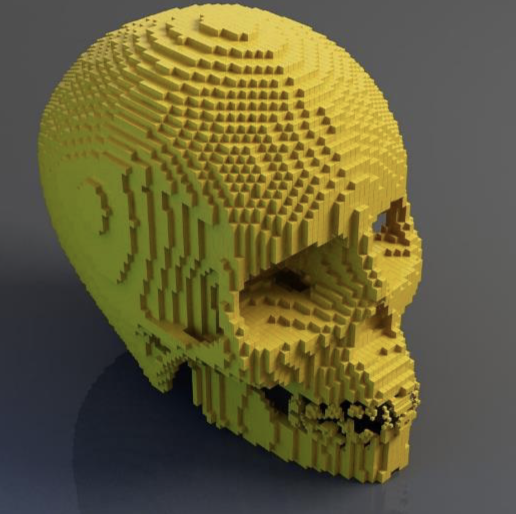
\includegraphics[width=100mm]{img/numeric.png}
	\caption{Пример изображения, полученного в результате 
		использования воксельного метода}
	\label{fig:numeric}
\end{figure}

Каждая ячейка при этом должна быть представлена основной 
характеристикой --- например, координатами центра.
При сканировании 
обычно устанавливается определённый порядок обхода, а соответствующий 
упорядоченный набор координат называется пространственным массивом.

Такие пространственные массивы помогают однозначно определить модель, т.е. построенная таким образом модель может быть получена только одним способом.
Пример изоображения, полученного в результате использования воксельного метода, представлен на рисунке \ref{fig:numeric}.

Недостатки:
\begin{itemize}[leftmargin=1.6\parindent]
	\item[---] большие затраты памяти;
	\item[---] каждая ячейка хранит информацию не только о своей координате, но и о цвете, плотности, оптических характеристиках и т. д.;
	\item[---] разрешение итогового изображения зависит от размера и формы вокселей.
\end{itemize}

Преимущества:
\begin{itemize}[leftmargin=1.6\parindent]
	\item[---] простота метода представления;
	\item[---] однозначность представления.
\end{itemize}

Простота и однозначность построения способствуют использованию 
данного метода при построении представлений, однако структурное 
использование кубических вокселей приводит к тому, что для рендера, например, сферы, будет необходимо проводить сглаживание краёв, что 
является дополнительной вычислительной нагрузкой.

В нашем случае недостатком является и избыточная информация о 
каждой ячейке.
Таким образом, самостоятельное использование данного метода 
является неэффективным, однако в совокупности с другими методами можно 
использовать преимущества аппроксимации для повышения качества 
изображения тела.

\subsubsection{Октантное дерево}

Данная схема представления является улучшением воксельного метода. 
Строится октантное дерево \cite{numeric-octree}, каждый узел которого соответствует некоторому 
кубу в трёхмерном пространстве, и для каждого куба определяется его 
принадлежность модели.
У каждого корня дерева есть 8 потомков, т.е. куб 
делится на 8 равных частей (пример подобного разделения представлен на рисунке \ref{fig:octTree}).

\begin{figure}[h]
	\centering
	\captionsetup{justification=centering}
	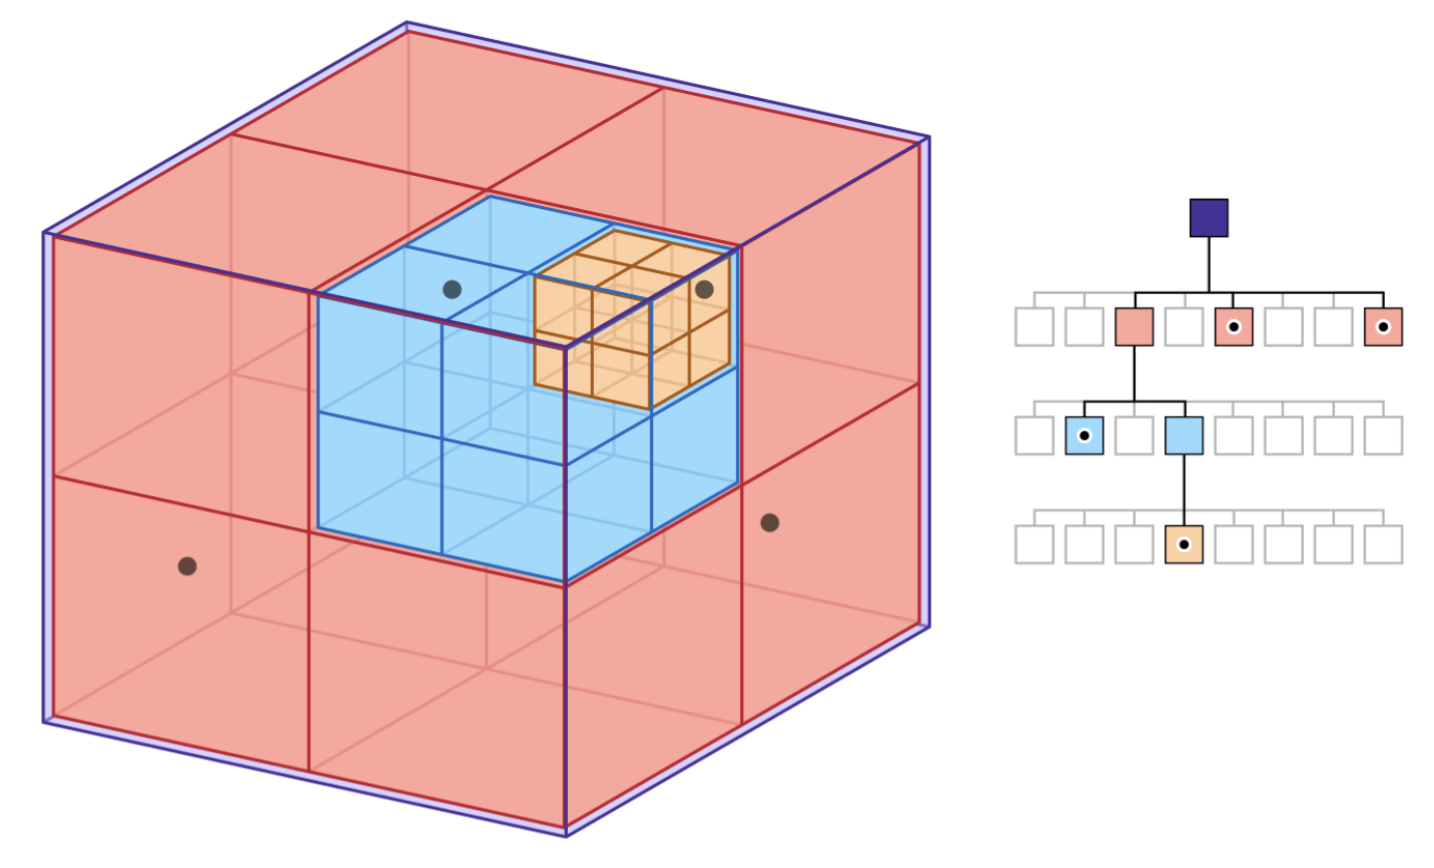
\includegraphics[width=\textwidth]{img/octTree.png}
	\caption{Разделение куба на 8 равных частей и получение 
		октантного дерева}
	\label{fig:octTree}
\end{figure}

Метод позволяет устранить недостаток метода \ref{sec:numeric}, 
связанного с затратами памяти из-за хранения большого количества данных.
И хотя, сохраняя данные только об используемых частях модели, данный метод экономит память в сравнении с воксельным, по отношению к другим методам, 
памяти расходуется много.

Недостатки:
\begin{itemize}[leftmargin=1.6\parindent]
	\item[---] деление примитива рёбрами кубов дерева может снижать 
	эффективность;
	\item[---] возможное выведение на экран невидимых объектов.
\end{itemize}

Преимущества:
\begin{itemize}[leftmargin=1.6\parindent]
	\item[---] простота метода представления;
	\item[---] однозначность представления.
\end{itemize}


\subsubsection{Выметание (Sweeping)}

Данный метод \cite{sweeping} позволяет получить трёхмерную модель из двумерной 
посредством движения по заданной траектории (sweep), например, движения 
вокруг заданной оси или относительно грани (пример использования выметания для получения трёхмерной модели представлен на рисунке \ref{fig:sweeping}).

\begin{figure}[h]
	\centering
	\captionsetup{justification=centering}
	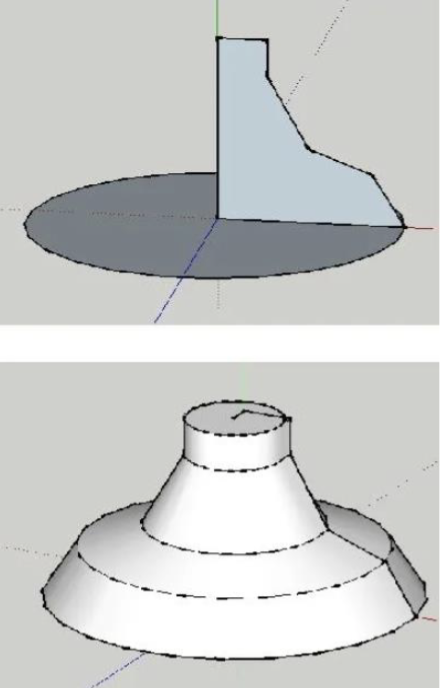
\includegraphics[width=64mm]{img/sweeping.png}
	\caption{Пример получения трёхмерного изображения посредством 
		вращения фигуры вокруг заданной оси}
	\label{fig:sweeping}
\end{figure}

Недостатком данного метода является необходимость задавать траектории движения 2D объектов, что может быть проблематично для тел, имеющих сложную форму.

К преимуществам выметания можно отнести удобство определения простых форм через простые плоские фигуры, а также возможность использования метода для быстрого удаления материала внутри тела (пример подобного использования выметания представлен на рисунке \ref{fig:deleting}). 
 
\begin{figure}[h]
	\centering
	\captionsetup{justification=centering}
	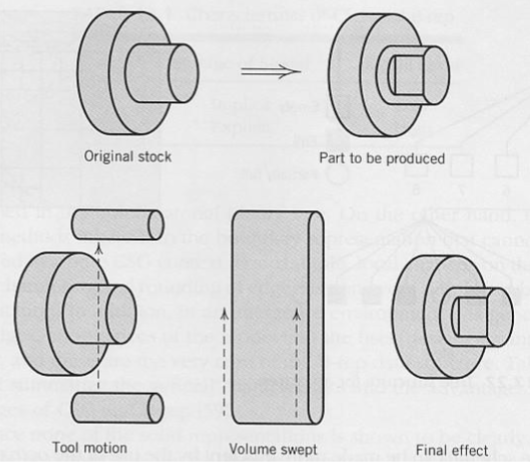
\includegraphics[width=80mm]{img/deleting.png}
	\caption{Пример удаления материала внутри тела посредством 
		алгоритма выметания}
	\label{fig:deleting}
\end{figure}


\subsubsection{Конструктивная блочная геометрия (CSG)}

Метод конструктивной блочной геометрии \cite{csg} основан на комбинировании 
примитивов посредством логических операций (объединения, пересечения, 
вычитания).
Любое составное тело может быть описано в виде традиционного 
уравнения из булевых функций, аргументами которого могут быть как 
примитивы, так и другие составные тела. 
Такое представление ещё называют 
деревом построений (пример дерева построений представлен на рисунке \ref{fig:csg}).
\newpage

\begin{figure}[h]
	\centering
	\captionsetup{justification=centering}
	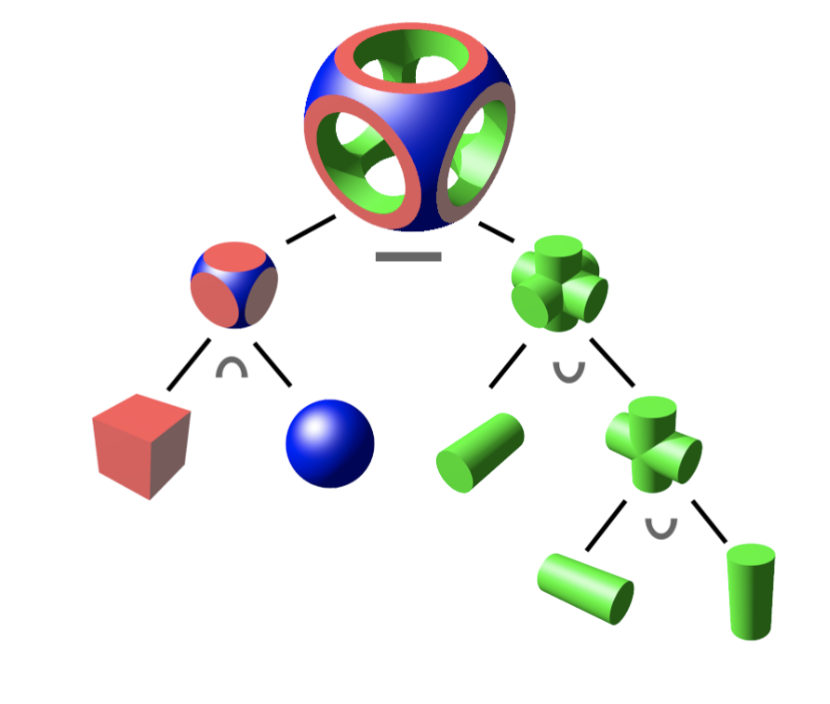
\includegraphics[width=90mm]{img/csg.png}
	\caption{Дерево построений при использовании CSG}
	\label{fig:csg}
\end{figure}


Особенностью данного метода является то, что необходимо учитывать 
возможное вырождение тела в плоское в результате логических операций.


\subsubsection{Сравение методов}

Сравним разобранные выше методы, разобрав их по нескольким 
критериям.
\begin{enumerate}[leftmargin=1.6\parindent,label=\arabic*.]
	\item Эффективность --- насколько много времени необходимо для создания, 
	исследования и изменения формы модели.
	\item Однозначность --- вместе с моделью хранятся данные, которых 
	достаточно для осуществления геометрических расчётов.
	\item Практичность --- создание модели без введения дополнительных 
	параметров, поддерживая удобство использования.
	\item Лаконичность --- сколько памяти компьютера занимает модель.
	\item Сохранность --- хранение истории преобразования модели, чтобы у 
	пользователя была возможность вернуться к предыдущему шагу 
	моделирования без использования преобразовательных вычислений.
	\item Уникальность --- возможность получить модель единственным способом.
\end{enumerate}

Разбор соответствующих критериев представлен в таблице \ref{table:presentation-1}.
\clearpage

\begin{table}[h]
\begin{center}
	\captionsetup{justification=centering}
	\begin{tabular}{| c | c | c | c | c | c | c |}
		\hline
		Метод & Эф-ть & Од-ть & Прак-ть & Лак-ть & Сох-ть & Ун-ть \\
		\hline
%		\begin{tabular}{c}
%			Клонирование\\
%			примитивов
%		\end{tabular} &$+$ & $+$ & $-$ & $-$ & $-$ & $-$ \\
%		\hline
		Brep & $+$ & $+$ & $-$ & $-$ & $-$ & $+$ \\
		\hline
		\begin{tabular}{c}
			Нумерация\\
			пространственного \\
			заполнения
		\end{tabular}  & $-$ & $+$ & $-$ & $-$ & $-$ & $+$ \\
		\hline
		Октантное дерево & $-$ & $+$ & $-$ & $+$ & $-$ & $+$ \\
		\hline
		Выметание & $-$ & $+$ & $-$ & $+$ & $-$ & $-$ \\
		\hline
		CSG & $+$ & $+$ & $+$ & $+$ & $+$ & $-$ \\
		\hline
	\end{tabular}
	\caption{Сравнительная таблица методов представления}
	\label{table:presentation-1}
\end{center}
\end{table}

После рассмотрения методов представления предлагается использовать 
CSG, как наиболее подходящий метод представления моделей.
Дерево построений 
является удобным с точки зрения модификации объекта и организации 
пользовательского интерфейса, обеспечивающего наглядный и быстрый доступ 
к любому элементу, входящему в описание геометрии тела.
Остальные схемы 
требуют дополнительную информацию, которая, хоть и является необходимой 
для представления модели, не требуется для решения поставленной задачи.

Недостатками выбранного метода является отсутствие высокой точности представляеомй модели и возможность получать одну и ту же модель несколькими способами, что не входит в требования, соответствующие поставленной задаче.


\subsection{Анализ методов рендера модели}

Рендеринг (англ. \textit{rendering} --- визуализация) --- термин, обозначающий 
процесс получения изображения по модели при помощи компьютерной 
программы. 
Рассмотрим различные методы рендера.

\subsubsection{Растеризация}

Растеризацией \cite{rasterization} называют процесс получения растрового изображения --- 
изображения, представляющего собой сетку пикселей --- цветных точек 
(обычно прямоугольных) на мониторе, бумаге или других отображающих 
устройствах.

Технология растеризации основана на обходе вершин треугольника, 
который после переноса из трёхмерного пространства в двумерное остаётся 
самим собой.
Каждая точка каждого обрабатываемого объекта в трёхмерном 
пространстве переводится в точку на экране, затем эти точки соединяются и 
получается изображение объекта.
На рисунке \ref{fig:rasterization} представлен пример переноса треугольлника из трёхмерного пространства в двумерное.

\begin{figure}[h]
	\centering
	\captionsetup{justification=centering}
	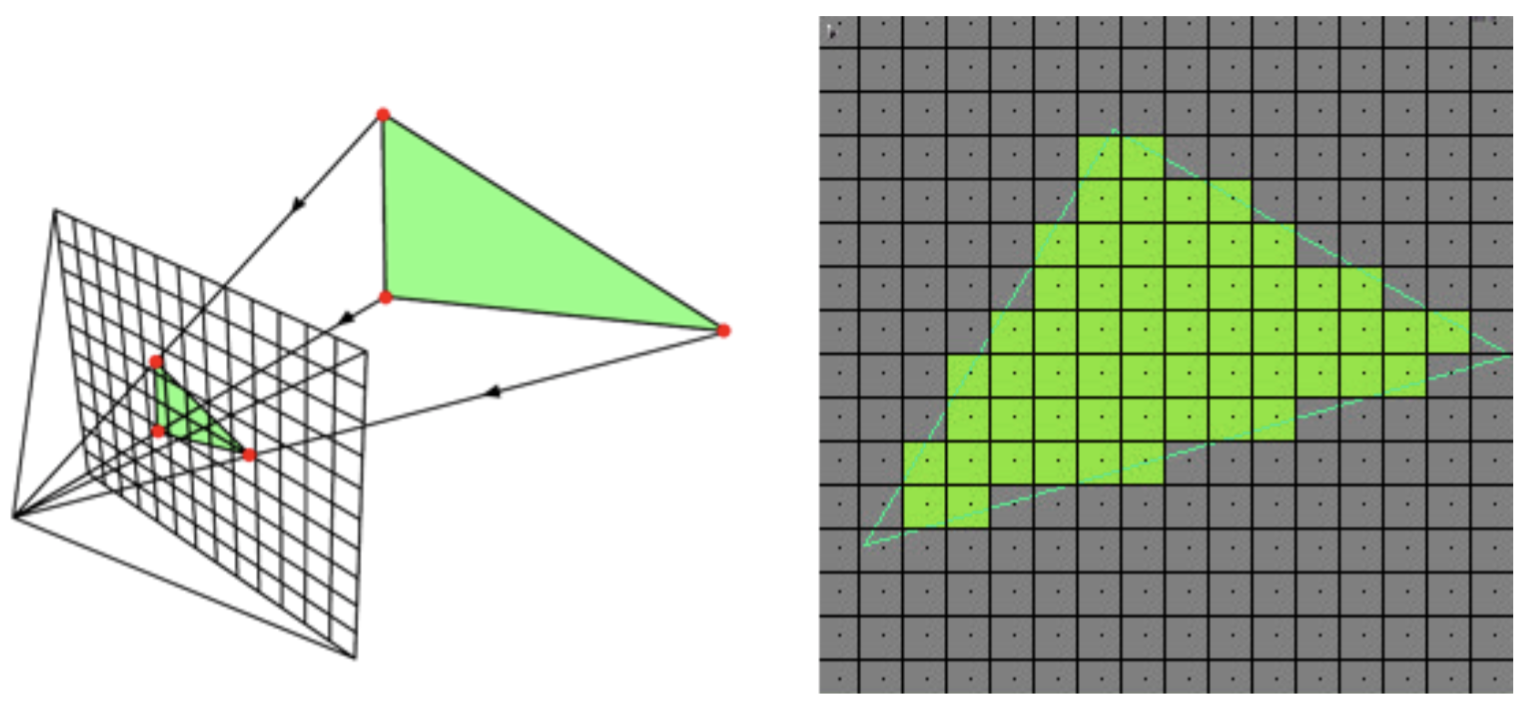
\includegraphics[width=130mm]{img/rasterization.png}
	\caption{Пример переноса треугольника из трёхмерного 
		пространства в двумерное}
	\label{fig:rasterization}
\end{figure}

Недостатки:
\begin{itemize}[leftmargin=1.6\parindent]
	\item[---] изображение может получиться «угловатым» (ступенчатым), что 
	потребует использования алгоритмов сглаживания;
	\item[---] алгоритм требует больших вычислительных ресурсов --- на дисплее 4К 
	примерно 8 миллионов пикселей, могут использоваться миллионы полигонов, 
	частота обновления кадров может быть высокой;
	\item[---] каждый пиксель обрабатывается много раз;
	\item[---] составные модели будет ресурсозатратно обрабатывать, т. к. 3D модель должна быть описана как набор примитивов.
\end{itemize}
\clearpage

Преимущества:
\begin{itemize}[leftmargin=1.6\parindent]
	\item[---] сравнительная простота алгоритма;
	\item[---] современные компьютеры оптимизированы для отрисовки растровых 
	изображений, что позволяет делать это довольно эффективно.
\end{itemize}

\subsubsection{Трассировка лучей}
Трассировка лучей (англ. \textit{Ray Tracing}) \cite{raytracing} --- технология отрисовки 
трёхмерной графики, симулирующая физическое поведение света. 

Одним из принципов трассировки лучей является поддержка 
совместимости с существующими трёхмерными моделями, большинство 
которых собрано из треугольников.
Для этого проверяется случай столкновения 
луча не со стеной, а с треугольником.
Рассмотрим этот случай.

Пусть вершины треугольника обозначаются как $V_0$, $V_1$, $V_2$. 
Векторы  двух его рёбер будут обозначены как $\vec{a}$, $\vec{b}$ и заданы формулами \ref{eq:a} и \ref{eq:b}
\begin{equation}
	\vec{a} = V_1 - V_0
	\label{eq:a}
\end{equation}
\begin{equation}
	\vec{b} = V_2 - V_0
	\label{eq:b}
\end{equation}

Определим луч $P$ c помощью параметрической формулы \ref{eq:p}:
\begin{equation}
	P= R_0 + t \cdot R_d
	\label{eq:p}
\end{equation}
где $R_0$ --- начальная точка луча, $R_d$ --- направление луча, $t$ --- расстояние вдоль луча до точки.

В плоскости треугольника точка пересечения будет иметь координаты $(u, v)$. Приравняв уравнение луча $P$ и плоскости в точке $(u, v)$, можно найти пересечение:
\begin{equation}
	P= V_0 + u \cdot \vec{a} + v \cdot \vec{b}
	\label{eq:p2}
\end{equation}

Таким образом, составив систему из трёх уравнений \ref{eq:rsys} для координат x, y, z и решив её для t, u, v, необходимо проанализировать определитель. Если 
он ненулевой (луч не параллелен плоскости), а $ t >= 0$ и u, v, u + v лежат в диапазоне от 0 до 1, то $P$ находится внутри треугольника и поиск столкновения завершается. Система \ref{eq:rsys}:

\begin{equation}
	\begin{cases}
		R_{0x} + t \cdot R_{dx} = V_{0x} + u \cdot A_x + v \cdot B_x \\
		R_{0y} + t \cdot R_{dy} = V_{0y} + u \cdot A_y + v \cdot B_y \\
		R_{0z} + t \cdot R_{dz} = V_{0z} + u \cdot A_z + v \cdot B_z \\
	\end{cases}
	\label{eq:rsys}
\end{equation}

Стоит учесть, что вычисления, связанные с конкретным лучом, могут не 
закончиться после одного треугольника: например, в случае отражения или 
преломления необходимо проследить дальнейшее поведение луча до тех пор, 
пока не произойдёт поглощение луча, возврат в начальную точку или превышение максимального числа отражений.

Несмотря на это, сложность алгоритма трассировки лучей позволяет получить более качественное изображение по сравнению с результатом, который может дать растеризация, за счёт отслеживания траектории лучей после отражения от объектов, а также учёта общей освещённости сцены (пример изображений, полученных в результате растеризации и трассировки лучей, представлен на рисунке \ref{fig:rasterisationVsRayTracing}).

\begin{figure}[h]
	\centering
	\captionsetup{justification=centering}
	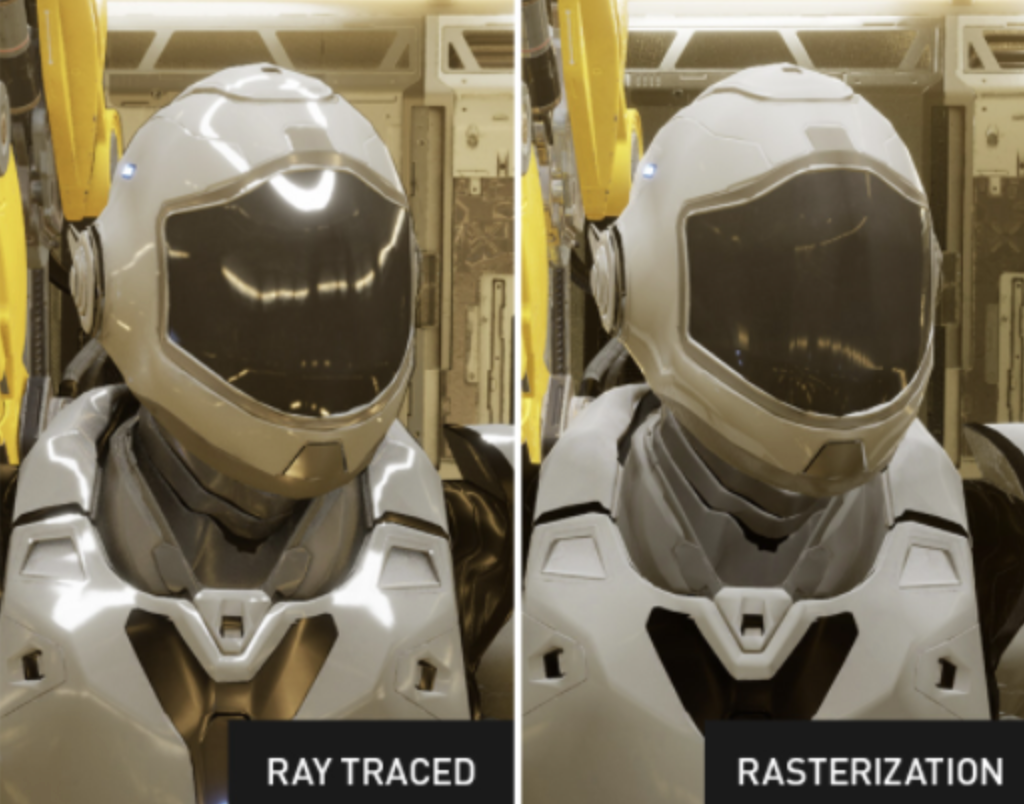
\includegraphics[width=90mm]{img/rasterisationVsRayTracing.png}
	\caption{Сравнение результатов работы алгоритмов растеризации и 
		трассировки лучей}
	\label{fig:rasterisationVsRayTracing}
\end{figure}

Недостатком данного метода является производительность (требуется большая вычислительная способность).


Преимущества:
\begin{itemize}[leftmargin=1.6\parindent]
	\item[---] возможность получать гладкие изображения без использования 
	дополнительных алгоритмов аппроксимации;
	\item[---] вычислительная сложность практически не зависит от сложности сцены;
	\item[---] отсечение невидимых поверхностей, изменение поля зрения и 
	перспективы являются частью алгоритма.
\end{itemize}

Несмотря на то, что данный алгоритм позволяет получать изображения 
хорошего качества, его использование требует больших мощностей.
Метод 
трассировки лучей каждый раз начинает процесс определения цвета пикселя 
заново, рассматривая каждый луч наблюдения отдельно.
Это позволяет придать 
изображению реалистичность и решает задачи отражения и преломления, 
однако требует много ресурсов.

\subsubsection{Бросание лучей}

Бросание лучей (англ. --- \textit{Ray Casting}) \cite{raycasting} --- это технология, позволяющая 
преобразовать набор данных в 3D проекцию посредством «бросания лучей» из 
точки обзора по всем областям видимости.

Идея алгоритма заключается в том, чтобы испускать лучи из камеры (глаз 
наблюдателя), по одному лучу на пиксель, после чего находить ближайший 
объект, который блокирует путь распространения данного луча.
Используя информацию о характеристиках материалов, алгоритм бросания лучей также может определять затенение объектов. 

Данная технология была достаточно распространена при создании игр в 
конце прошлого века, а из-за возможности преобразования чего-то двумерного 
в что-то почти трёхмерное графические изображения, полученные в результате 
бросания лучей, часто называли «псевдо 3D» или «2.5D».
Пример работы алгоритма бросания лучей приведён на рисунке \ref{fig:raycasting}.

\begin{figure}[h]
	\centering
	\captionsetup{justification=centering}
	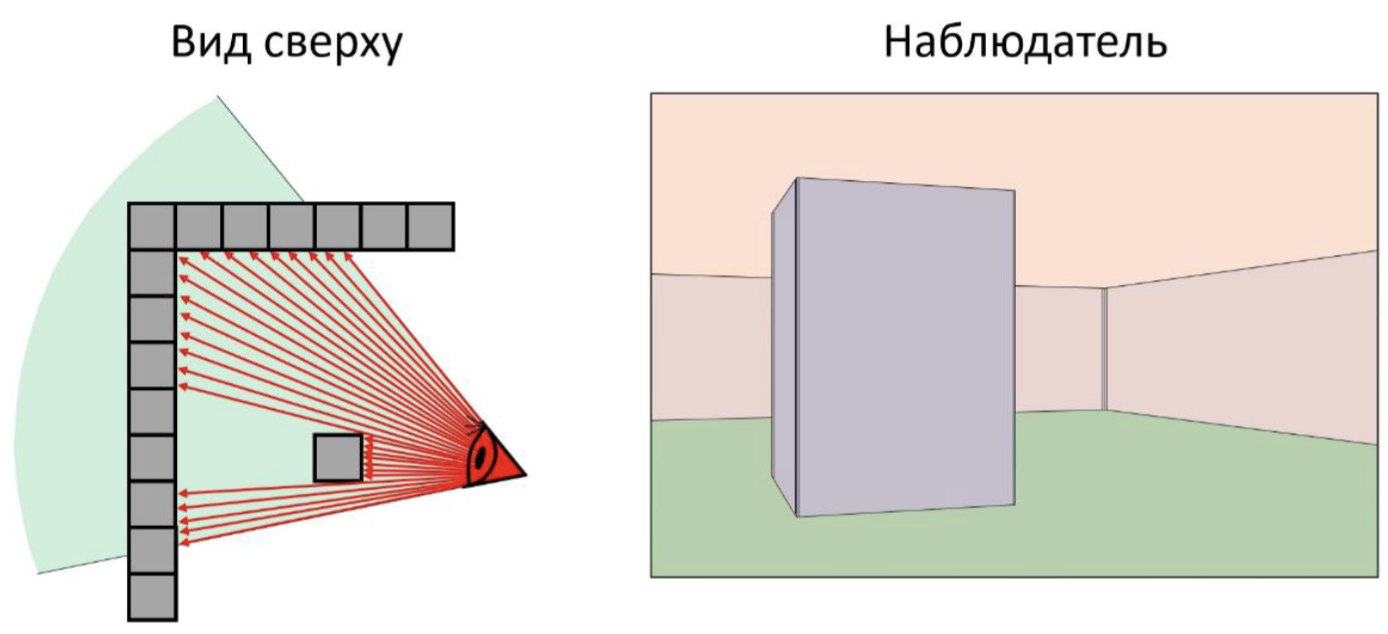
\includegraphics[width=150mm]{img/raycasting.png}
	\caption{Пример работы алгоритма бросания лучей}
	\label{fig:raycasting}
\end{figure}

Недостатки:
\begin{itemize}[leftmargin=1.6\parindent]
	\item[---] в результате рендера получается изображение средне-плохого качества по сравнению с другими методами;
	\item[---] есть геометрические ограничения, накладываемые на обрабатываемую поверхность (только простые фигуры).
\end{itemize}

Преимущества:
\begin{itemize}[leftmargin=1.6\parindent]
	\item[---] простота реализации алгоритма;
	\item[---] низкие требования к вычислениям;
	\item[---] возможность получать изображение с течением времени («на лету»).
\end{itemize}

Из-за указанных геометрических ограничений у игр, созданных с 
использованием технологии бросания лучей, было множество недостатков: 
потолок был одной высоты, не было никаких трёхмерных объектов, кроме 
потолка, стен и пола, всё остальное — двумерные изображения в трёхмерном 
пространстве (пример подобной игры представлен на рисунке \ref{fig:doom}). \clearpage

\begin{figure}[h]
	\centering
	\captionsetup{justification=centering}
	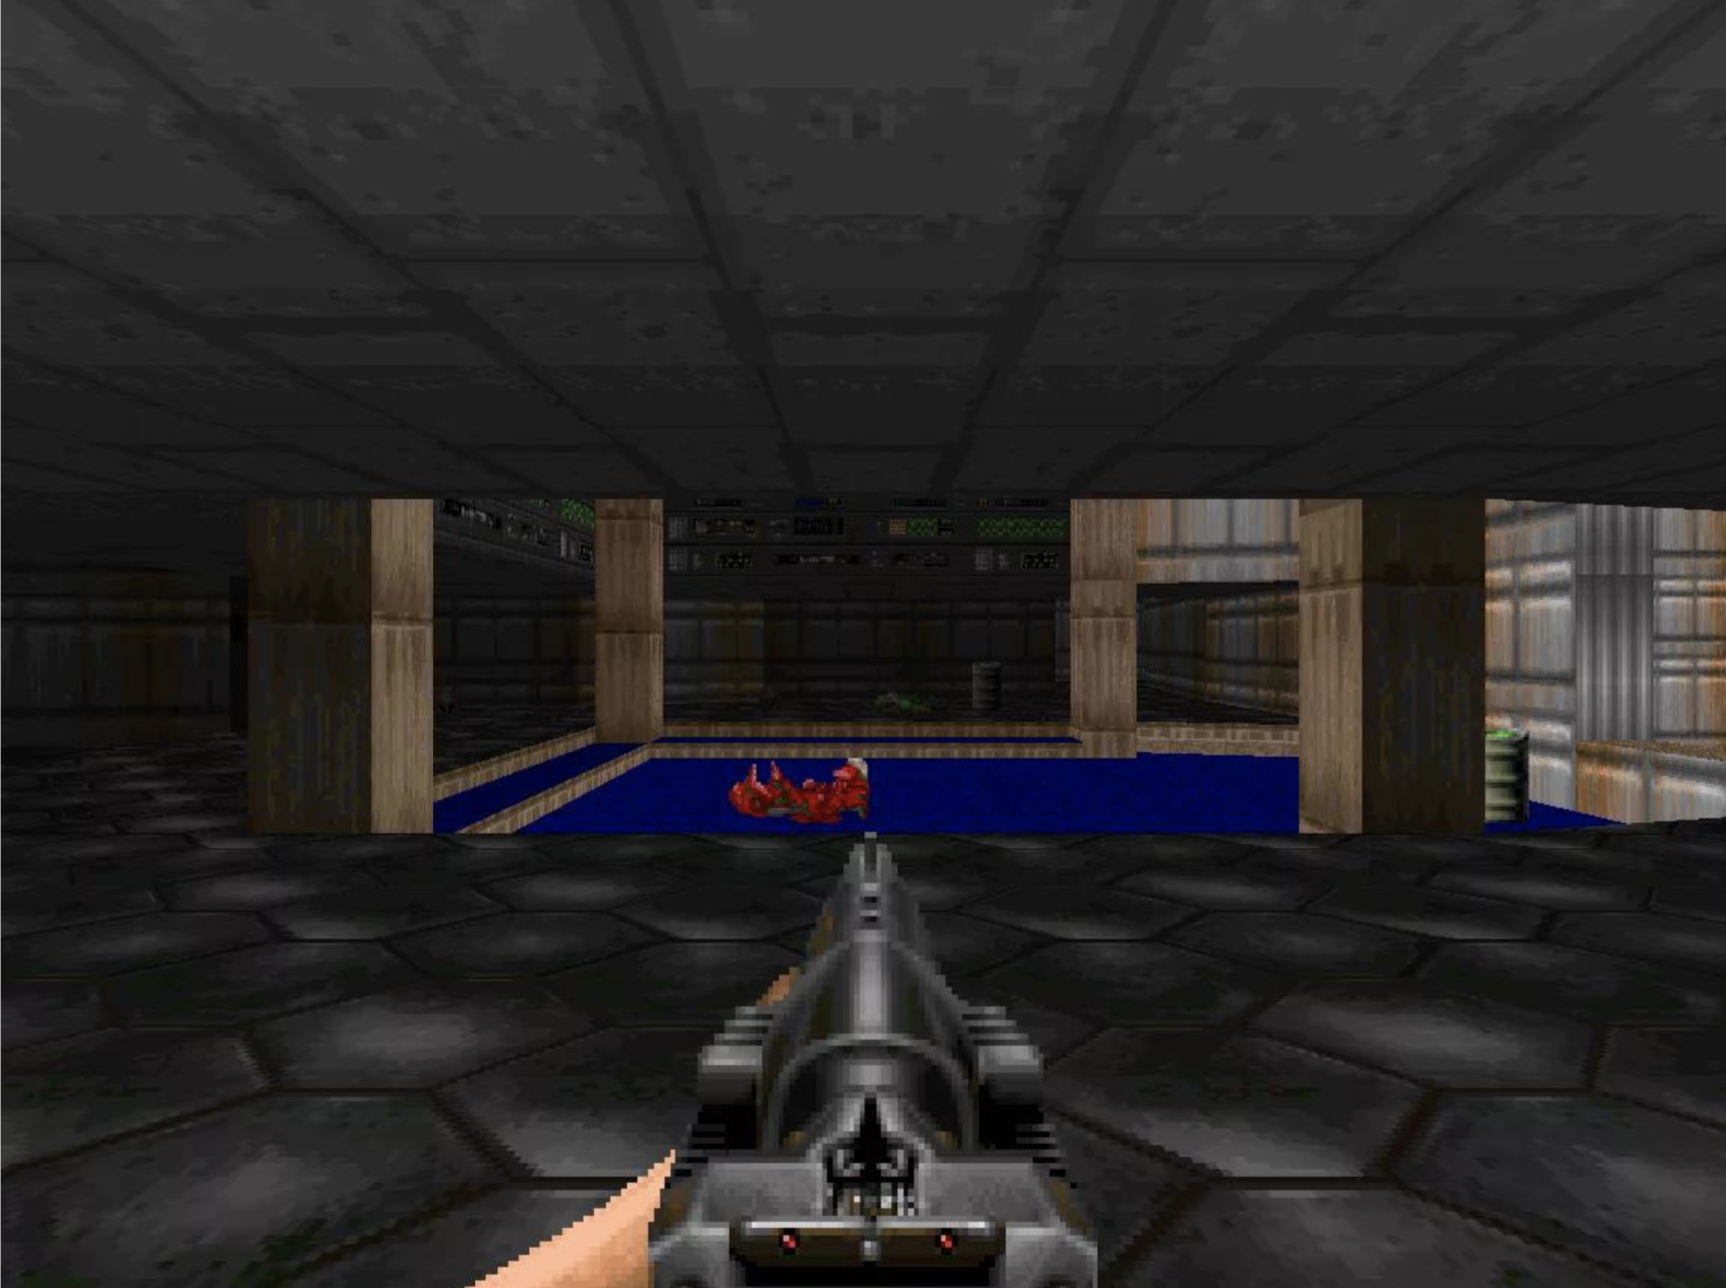
\includegraphics[width=120mm]{img/doom.png}
	\caption{Скриншот из игры Doom 1: Объекты (оружие и противники) --- 
		просто растровые изображения, перенесённые и отрисованные поверх фона}
	\label{fig:doom}
\end{figure}


\subsubsection{Марширование лучей}
Марширование лучей (англ. \textit{Ray Marching}) \cite{raymarching} --- разновидность алгоритмов 
трассировки лучей, является изменённой версией технологии Ray Tracing.

Ray Marching похож на традиционную технологию трассировки лучей 
тем, что лучи в сцену испускаются для каждого пикселя.
Однако в то время, как 
в трассировке лучей имеются системы уравнений, позволяющие получить 
точку пересечения луча и объектов, в технологии марширования лучей 
предлагается другое решение.

Происходит смещение текущего положения вдоль луча до тех пор, пока не будет найдена точка, пересекающая 
объект.
Данная операция является простой по сравнению с решением системы 
уравнений, однако находит точку пересечения не слишком точно. 
На рисунке \ref{fig:raymarchingfixed} продемонстрирован пример простейшей реализации марширования лучей с фиксированным интервалом шага (красными точками отмечены все обрабатываемые точки).

\clearpage

\begin{figure}[h]
	\centering
	\captionsetup{justification=centering}
	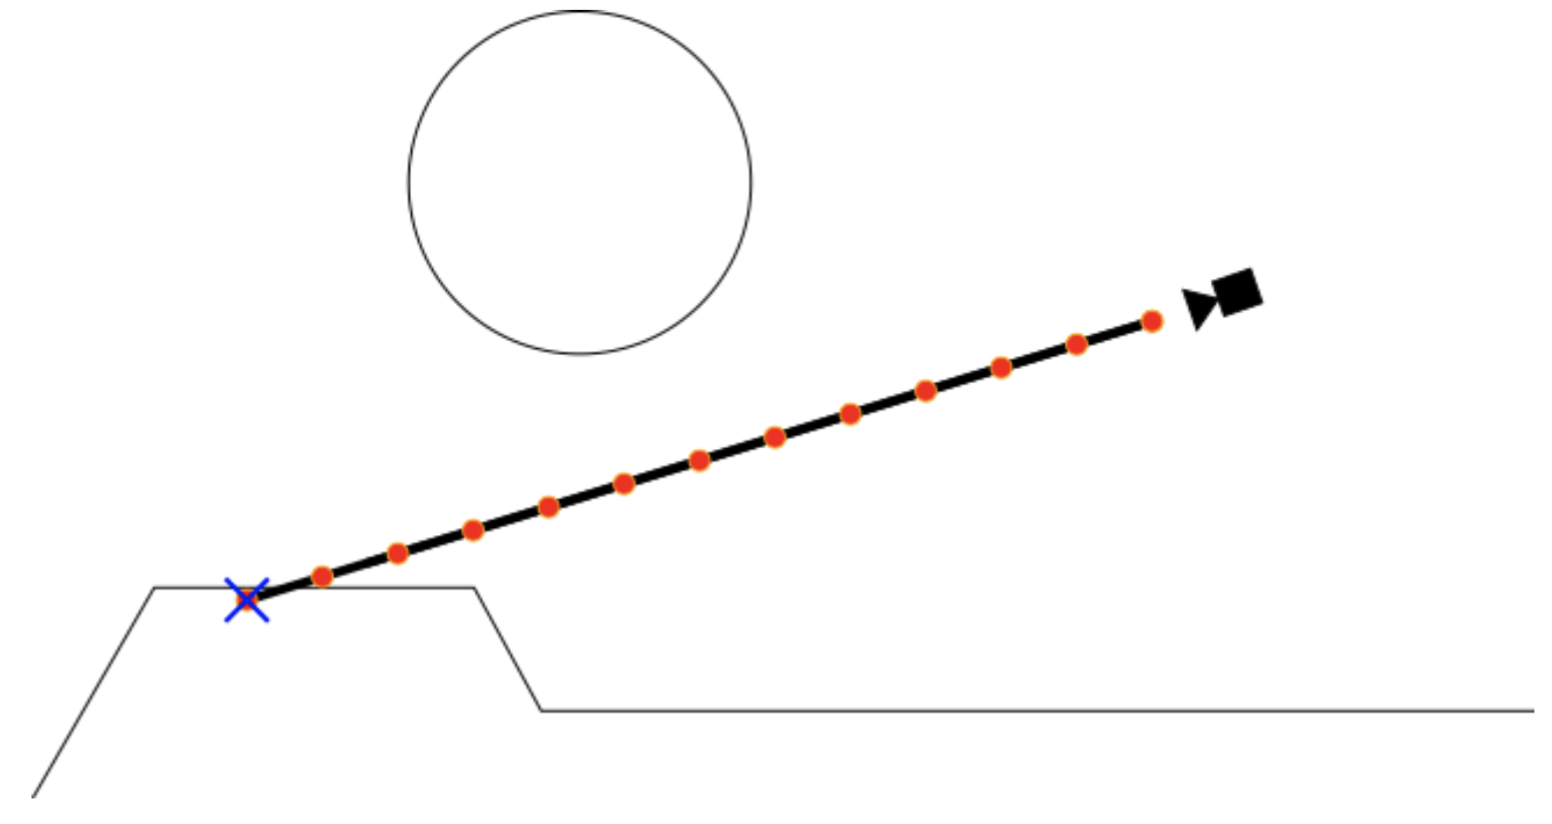
\includegraphics[width=110mm]{img/raymarchingfixed.png}
	\caption{Простейшая реализация метода Ray Marching с фиксированным интервалом шага}
	\label{fig:raymarchingfixed}
\end{figure}

Данная реализация вполне достаточна для использования во множестве 
областей, например, в случаях построения объёмных и прозрачных 
поверхностей.
Для непрозрачных объектов можно ввести ещё одну 
оптимизацию, для которой будет использовано поле расстояний со знаком.

Поле расстояний со знаком (англ. \textit{Signed Distance Field}) — это функция, 
получающая на входе координаты точки и возвращающая кратчайшее 
расстояние от этой точки до поверхности каждого объекта в сцене.
При этом возвращается отрицательное число, если точка находится внутри объекта.
Таким образом, мы можем ограничить количество шагов при движении вдоль 
луча.

Описание алгоритма: для каждого пикселя на экране определяется 
расстояние до ближайшего объекта, которое позволяет получить радиус, на который 
можно пустить луч. 
Для конечной точки луча определяем радиус до тех пор, 
пока он не станет достаточно маленьким --- это будет означать столкновение с 
объектом.
Если же радиус стабильно увеличивается, то это показывает, что луч 
прошёл мимо объектов на сцене.
На рисунке \ref{fig:raymarchingsdf} продемонстрирована визуализация метода марширования лучей с использованием SDF. Красным цветом отвечены обрабатываемые точки, синим цветом --- области, которые гарантированно не содержат объектов, пунктирными зелёными линиями --- истинные кратчайшие векторы между каждой обрабатываемой точкой и сценой.


\begin{figure}[h]
	\centering
	\captionsetup{justification=centering}
	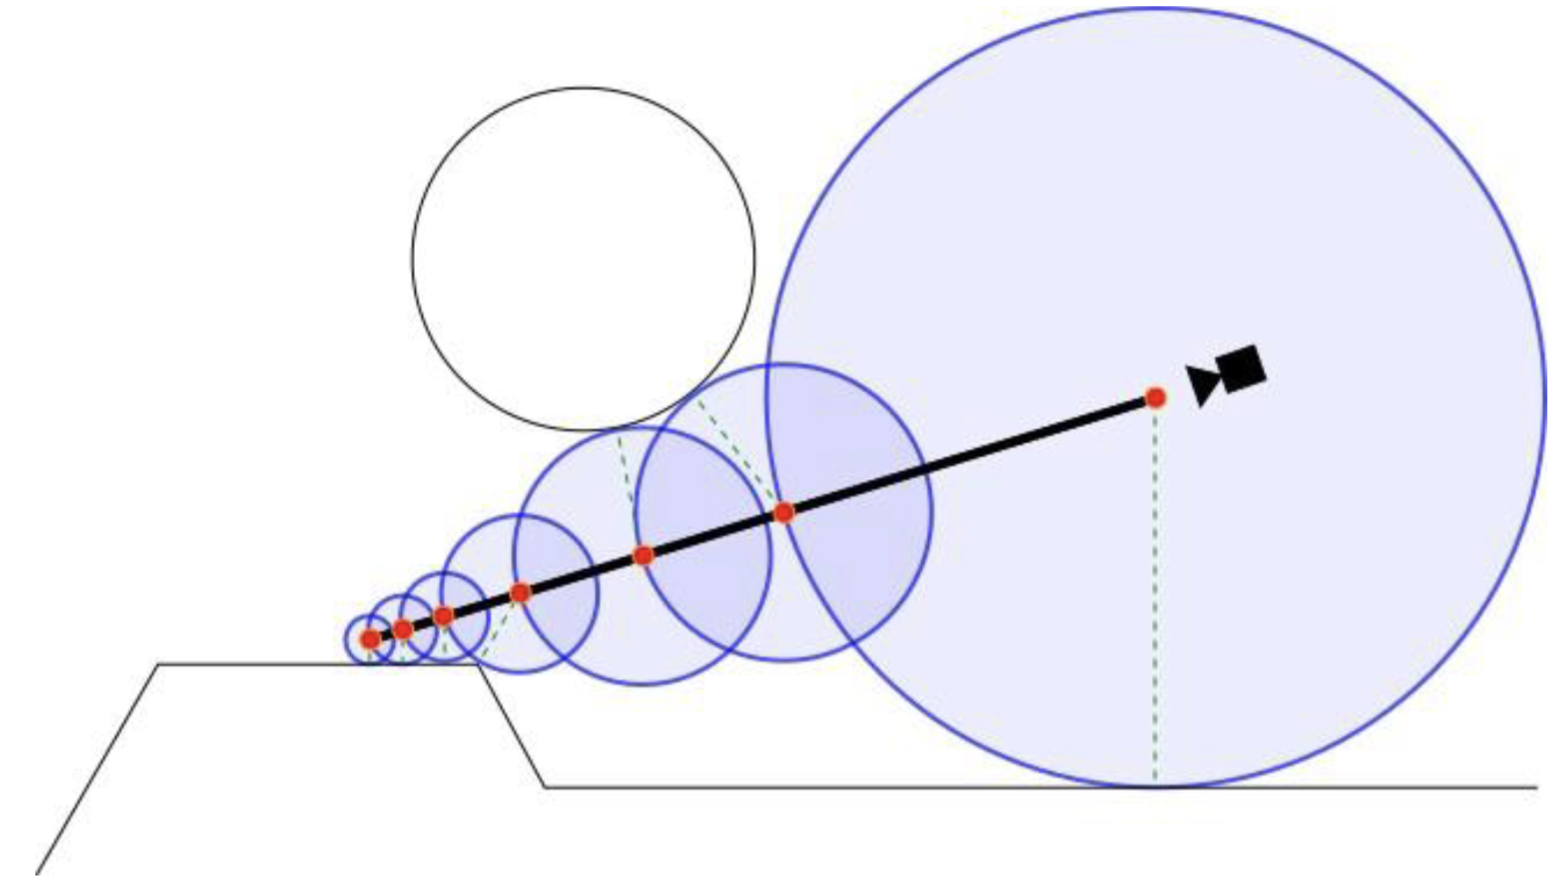
\includegraphics[width=120mm]{img/raymarchingsdf.png}
	\caption{Визуализация метода RayMarching с использованием поля расстояний со знаком}
	\label{fig:raymarchingsdf}
\end{figure}

Недостатком данного алгоритма является неточность найденного значения координат пересечения луча и объекта.

Преимущества:
\begin{itemize}[leftmargin=1.6\parindent]
	\item[---] неплохая производительность по сравнению с технологией трассировки лучей;
	\item[---] метод подходит для рендера сложных поверхностей, для которых 
	сложно определить пересечение аналитическими методами;
	\item[---] используя поля расстояний со знаком можно произвести ускорение    
	рендеринга до реального времени;
	\item[---] хорошее качество изображения (сопоставимое с результатами алгоритма трассировки лучей).     
\end{itemize}
%\clearpage  

\subsubsection{Сравнение методов}

Сравним разобранные выше методы, разобрав их по нескольким 
критериям.
\begin{enumerate}[leftmargin=1.6\parindent,label=\arabic*.]
	\item Быстродействие, т.е. как много времени нужно для рендера модели.
	\item Точность, т.е. обработка истинных границ рассматриваемой модели.
	\item Качество получаемого изображения.
	\item Реальность — возможность работы в режиме 
	реального времени.
\end{enumerate}

Разбор соответствующих критериев представлен в таблице \ref{table:presentation}

\begin{table}[h]
	\begin{center}
		\captionsetup{justification=centering}
		\begin{tabular}{| c | c | c | c | c |}
			\hline
			Метод & Быстродействие & Точность & Качество & Реальность \\
			\hline
			Растеризация &$+$ & $+$ & $-$ & $+$\\
			\hline
			Ray Tracing & $-$ & $+$ & $+$ & $-$\\
			\hline
			Ray Casting  & $+$ & $+$ & $-$ & $+$\\
			\hline
			Ray Marching & $+$ & $-$ & $+$ & $+$\\
			\hline
		\end{tabular}
		\caption{Сравнительная таблица методов рендера}
		\label{table:presentation}
	\end{center}
\end{table}

Таким образом, были рассмотрены методы рендера модели.
Учитывая поставленную задачу, а также метод представления модели, выбранный в предыдущем разделе, можно сказать, что алгоритм марширования лучей (Ray Marching) является оптимальным при использовании конструктивной 
блочной геометрии (CSG). 
В такой связке можно получать качественное 
изображение при отрисовке в режиме реального времени.
Есть и недостаток такого выбора: будет присутствовать некоторая погрешность при вычислении границ объекта.

\subsection{Методы преобразования и визуализации}

В данном разделе рассматриваются способы преобразования модели и 
придания ей реалистичного вида.

\subsubsection{Матрицы преобразования}

Для преобразования тела в пространстве обычно используются операции 
перемещения, поворота и масштабирования.
Осуществление этих преобразований может быть реализовано при помощи матриц преобразования \cite{transformations} (таблица \ref{table:matrix}).

\begin{table}[ht]
	\small
	\captionsetup{justification=centering}
	\caption{Таблица преобразований}
	\begin{tabular}{|l|c|l|}
		\hline
		Преобразование & Матрица & Формула\\
		\hline
		Перемещение      & $\begin{pmatrix}
			1  & 0  & 0  & 0 \\
			0  & 1  & 0  & 0 \\
			0  & 0  & 1  & 0 \\
			dx & dy & dz & 1
		\end{pmatrix}$  & $\begin{cases}
			x_1=x+dx \\
			y_1=y+dy \\
			z_1=z+dz
		\end{cases}$  \\
		\hline
		Масштаб - е  & $\begin{pmatrix}
			k_x & 0   & 0   & 0 \\
			0   & k_y & 0   & 0 \\
			0   & 0   & k_z & 0 \\
			0   & 0   & 0   & 1
		\end{pmatrix}$ & $\begin{cases}
			x_1=k_x+(1-k_x)x_m \\
			y_1=k_y+(1-k_y)y_m \\
			z_1=k_z+(1-k_z)z_m
		\end{cases}$ \\
		\hline
		Поворот OX & $\begin{pmatrix}
			1 & 0           & 0          & 0 \\
			0 & \cos\theta  & \sin\theta & 0 \\
			0 & -\sin\theta & \cos\theta & 0 \\
			0 & 0           & 0          & 1
		\end{pmatrix}$ & $\begin{cases}
			x_1=x                                       \\
			y_1=y_c+(y-y_c)\cos\theta-(z-z_c)\sin\theta \\
			z_1=z_c+(y-y_c)\sin\theta+(z-z_c)\cos\theta
		\end{cases}$ \\
		\hline
		Поворот OY & $\begin{pmatrix}
			\cos\theta & 0 & -\sin\theta & 0 \\
			0          & 1 & 0           & 0 \\\sin\theta&0&\cos\theta&0 \\
			0          & 0 & 0           & 1
		\end{pmatrix}$ & $\begin{cases}
			x_1=x_c+(x-x_c)\cos\theta+(z-z_c)\sin\theta \\
			y_1=y \\
			z_1=z_c-(x-x_c)\sin\theta+(z-z_c)\cos\theta
		\end{cases}$ \\
		\hline
		Поворот OZ & $\begin{pmatrix}
			\cos\theta  & \sin\theta & 0 & 0 \\
			-\sin\theta & \cos\theta & 0 & 0 \\
			0           & 0          & 1 & 0 \\
			0           & 0          & 0 & 1
		\end{pmatrix}$ & $\begin{cases}
			x_1=x_c+(x-x_c)\cos\theta-(y-y_c)\sin\theta \\
			y_1=y_c+(x-x_c)\sin\theta+(y-y_c)\cos\theta \\
			z_1=z
		\end{cases}$ \\
		\hline
	\end{tabular}
	\label{table:matrix}
\end{table}
\clearpage

Происходит  умножение  исходных  координат  объекта  на  одну  или 
несколько  матриц,  в  результате  чего  происходит  перемещение, поворот  или 
масштабирование  объекта  в  зависимости  от  применённых  преобразований.
Матрицы  позволяют  перевести  координаты  модели  в мировые  координаты,  настроить  перспективу,  а  также  переместить  сцену 
относительно камеры. 

\subsubsection{Шейдеры}
Шейдером  называют  компьютерную  программу,  предназначенную  для 
исполнения процессорами видеокарты (GPU).

В разрабатываемом приложении использование шейдеров необходимо для 
придания изображению трёхмерного вида (используя тени и освещение).
Для этого существуют два вида шейдеров: фрагментные и вершинные \cite{shaders}.

Фрагментные  шейдеры  работают  с  конкретными  пикселями  объекта  и 
управляют их цветом. 
Работа фрагментного шейдера в графической обработке 
происходит после выполнения работы вершинным шейдером и влияет только на 
цветовую составляющую, преобразуя вершины в пиксели определённого цвета.

Вершинные  шейдеры  работают  с  вершинами  (из  списка  вершин)  и 
отображают  их  в  пространстве.
Шейдеру  передаются  три  матрицы:  матрица модели, матрица вида и матрица проекции.
Матрица  модели  необходима  для  перехода  от  пространства  модели,  в 
котором  координаты  вершин  определены  относительно  центра  модели,  в 
мировое пространство (в котором все вершины определены относительно центра 
мира).

Матрица вида используется для перемещения сцены относительно камеры.
В реальном мире происходит перемещение камеры относительно сцены, однако 
в  компьютерной  графике  проще  и  удобнее  переместить  сцену 
относительно камеры.

Матрица  проекции  позволяет  представить  перспективу  камеры.
При умножении координат на данную матрицу происходит сопоставление вершины с перспективой камеры, её соотношению сторон и полю обзора.




Итак, в данном разделе были рассмотрены методы преобразования модели 
--- матрицы  преобразования,  а  также  методы  преобразования  плоского 
изображения в трёхмерный вид --- шейдеры (вершинные и фрагментные). 

\subsection*{Вывод}
В  данной  главе  был  проведён  анализ  возможных  методов  для  решения 
поставленной задачи.
Как метод представления  модели, при помощи которой будет 
решаться поставленная задача,  была  выбрана  конструктивная  блочная геометрия  (CSG), 
рендера  ---  Ray Marching.
Для  преобразования  модели  будут  использоваться 
матрицы преобразований, для придания им трёхмерного вида --- шейдеры.
